% Options for packages loaded elsewhere
% Options for packages loaded elsewhere
\PassOptionsToPackage{unicode}{hyperref}
\PassOptionsToPackage{hyphens}{url}
\PassOptionsToPackage{dvipsnames,svgnames,x11names}{xcolor}
%
\documentclass[
  11pt,
  a4paper,
  openany]{scrreprt}
\usepackage{xcolor}
\usepackage[left=3cm,right=2.5cm,top=3cm,bottom=3cm]{geometry}
\usepackage{amsmath,amssymb}
\setcounter{secnumdepth}{2}
\usepackage{iftex}
\ifPDFTeX
  \usepackage[T1]{fontenc}
  \usepackage[utf8]{inputenc}
  \usepackage{textcomp} % provide euro and other symbols
\else % if luatex or xetex
  \usepackage{unicode-math} % this also loads fontspec
  \defaultfontfeatures{Scale=MatchLowercase}
  \defaultfontfeatures[\rmfamily]{Ligatures=TeX,Scale=1}
\fi
\usepackage{lmodern}
\ifPDFTeX\else
  % xetex/luatex font selection
\fi
% Use upquote if available, for straight quotes in verbatim environments
\IfFileExists{upquote.sty}{\usepackage{upquote}}{}
\IfFileExists{microtype.sty}{% use microtype if available
  \usepackage[]{microtype}
  \UseMicrotypeSet[protrusion]{basicmath} % disable protrusion for tt fonts
}{}
\makeatletter
\@ifundefined{KOMAClassName}{% if non-KOMA class
  \IfFileExists{parskip.sty}{%
    \usepackage{parskip}
  }{% else
    \setlength{\parindent}{0pt}
    \setlength{\parskip}{6pt plus 2pt minus 1pt}}
}{% if KOMA class
  \KOMAoptions{parskip=half}}
\makeatother
% Make \paragraph and \subparagraph free-standing
\makeatletter
\ifx\paragraph\undefined\else
  \let\oldparagraph\paragraph
  \renewcommand{\paragraph}{
    \@ifstar
      \xxxParagraphStar
      \xxxParagraphNoStar
  }
  \newcommand{\xxxParagraphStar}[1]{\oldparagraph*{#1}\mbox{}}
  \newcommand{\xxxParagraphNoStar}[1]{\oldparagraph{#1}\mbox{}}
\fi
\ifx\subparagraph\undefined\else
  \let\oldsubparagraph\subparagraph
  \renewcommand{\subparagraph}{
    \@ifstar
      \xxxSubParagraphStar
      \xxxSubParagraphNoStar
  }
  \newcommand{\xxxSubParagraphStar}[1]{\oldsubparagraph*{#1}\mbox{}}
  \newcommand{\xxxSubParagraphNoStar}[1]{\oldsubparagraph{#1}\mbox{}}
\fi
\makeatother

\usepackage{color}
\usepackage{fancyvrb}
\newcommand{\VerbBar}{|}
\newcommand{\VERB}{\Verb[commandchars=\\\{\}]}
\DefineVerbatimEnvironment{Highlighting}{Verbatim}{commandchars=\\\{\}}
% Add ',fontsize=\small' for more characters per line
\usepackage{framed}
\definecolor{shadecolor}{RGB}{241,243,245}
\newenvironment{Shaded}{\begin{snugshade}}{\end{snugshade}}
\newcommand{\AlertTok}[1]{\textcolor[rgb]{0.68,0.00,0.00}{#1}}
\newcommand{\AnnotationTok}[1]{\textcolor[rgb]{0.37,0.37,0.37}{#1}}
\newcommand{\AttributeTok}[1]{\textcolor[rgb]{0.40,0.45,0.13}{#1}}
\newcommand{\BaseNTok}[1]{\textcolor[rgb]{0.68,0.00,0.00}{#1}}
\newcommand{\BuiltInTok}[1]{\textcolor[rgb]{0.00,0.23,0.31}{#1}}
\newcommand{\CharTok}[1]{\textcolor[rgb]{0.13,0.47,0.30}{#1}}
\newcommand{\CommentTok}[1]{\textcolor[rgb]{0.37,0.37,0.37}{#1}}
\newcommand{\CommentVarTok}[1]{\textcolor[rgb]{0.37,0.37,0.37}{\textit{#1}}}
\newcommand{\ConstantTok}[1]{\textcolor[rgb]{0.56,0.35,0.01}{#1}}
\newcommand{\ControlFlowTok}[1]{\textcolor[rgb]{0.00,0.23,0.31}{\textbf{#1}}}
\newcommand{\DataTypeTok}[1]{\textcolor[rgb]{0.68,0.00,0.00}{#1}}
\newcommand{\DecValTok}[1]{\textcolor[rgb]{0.68,0.00,0.00}{#1}}
\newcommand{\DocumentationTok}[1]{\textcolor[rgb]{0.37,0.37,0.37}{\textit{#1}}}
\newcommand{\ErrorTok}[1]{\textcolor[rgb]{0.68,0.00,0.00}{#1}}
\newcommand{\ExtensionTok}[1]{\textcolor[rgb]{0.00,0.23,0.31}{#1}}
\newcommand{\FloatTok}[1]{\textcolor[rgb]{0.68,0.00,0.00}{#1}}
\newcommand{\FunctionTok}[1]{\textcolor[rgb]{0.28,0.35,0.67}{#1}}
\newcommand{\ImportTok}[1]{\textcolor[rgb]{0.00,0.46,0.62}{#1}}
\newcommand{\InformationTok}[1]{\textcolor[rgb]{0.37,0.37,0.37}{#1}}
\newcommand{\KeywordTok}[1]{\textcolor[rgb]{0.00,0.23,0.31}{\textbf{#1}}}
\newcommand{\NormalTok}[1]{\textcolor[rgb]{0.00,0.23,0.31}{#1}}
\newcommand{\OperatorTok}[1]{\textcolor[rgb]{0.37,0.37,0.37}{#1}}
\newcommand{\OtherTok}[1]{\textcolor[rgb]{0.00,0.23,0.31}{#1}}
\newcommand{\PreprocessorTok}[1]{\textcolor[rgb]{0.68,0.00,0.00}{#1}}
\newcommand{\RegionMarkerTok}[1]{\textcolor[rgb]{0.00,0.23,0.31}{#1}}
\newcommand{\SpecialCharTok}[1]{\textcolor[rgb]{0.37,0.37,0.37}{#1}}
\newcommand{\SpecialStringTok}[1]{\textcolor[rgb]{0.13,0.47,0.30}{#1}}
\newcommand{\StringTok}[1]{\textcolor[rgb]{0.13,0.47,0.30}{#1}}
\newcommand{\VariableTok}[1]{\textcolor[rgb]{0.07,0.07,0.07}{#1}}
\newcommand{\VerbatimStringTok}[1]{\textcolor[rgb]{0.13,0.47,0.30}{#1}}
\newcommand{\WarningTok}[1]{\textcolor[rgb]{0.37,0.37,0.37}{\textit{#1}}}

\usepackage{longtable,booktabs,array}
\usepackage{calc} % for calculating minipage widths
% Correct order of tables after \paragraph or \subparagraph
\usepackage{etoolbox}
\makeatletter
\patchcmd\longtable{\par}{\if@noskipsec\mbox{}\fi\par}{}{}
\makeatother
% Allow footnotes in longtable head/foot
\IfFileExists{footnotehyper.sty}{\usepackage{footnotehyper}}{\usepackage{footnote}}
\makesavenoteenv{longtable}
\usepackage{graphicx}
\makeatletter
\newsavebox\pandoc@box
\newcommand*\pandocbounded[1]{% scales image to fit in text height/width
  \sbox\pandoc@box{#1}%
  \Gscale@div\@tempa{\textheight}{\dimexpr\ht\pandoc@box+\dp\pandoc@box\relax}%
  \Gscale@div\@tempb{\linewidth}{\wd\pandoc@box}%
  \ifdim\@tempb\p@<\@tempa\p@\let\@tempa\@tempb\fi% select the smaller of both
  \ifdim\@tempa\p@<\p@\scalebox{\@tempa}{\usebox\pandoc@box}%
  \else\usebox{\pandoc@box}%
  \fi%
}
% Set default figure placement to htbp
\def\fps@figure{htbp}
\makeatother


% definitions for citeproc citations
\NewDocumentCommand\citeproctext{}{}
\NewDocumentCommand\citeproc{mm}{%
  \begingroup\def\citeproctext{#2}\cite{#1}\endgroup}
\makeatletter
 % allow citations to break across lines
 \let\@cite@ofmt\@firstofone
 % avoid brackets around text for \cite:
 \def\@biblabel#1{}
 \def\@cite#1#2{{#1\if@tempswa , #2\fi}}
\makeatother
\newlength{\cslhangindent}
\setlength{\cslhangindent}{1.5em}
\newlength{\csllabelwidth}
\setlength{\csllabelwidth}{3em}
\newenvironment{CSLReferences}[2] % #1 hanging-indent, #2 entry-spacing
 {\begin{list}{}{%
  \setlength{\itemindent}{0pt}
  \setlength{\leftmargin}{0pt}
  \setlength{\parsep}{0pt}
  % turn on hanging indent if param 1 is 1
  \ifodd #1
   \setlength{\leftmargin}{\cslhangindent}
   \setlength{\itemindent}{-1\cslhangindent}
  \fi
  % set entry spacing
  \setlength{\itemsep}{#2\baselineskip}}}
 {\end{list}}
\usepackage{calc}
\newcommand{\CSLBlock}[1]{\hfill\break\parbox[t]{\linewidth}{\strut\ignorespaces#1\strut}}
\newcommand{\CSLLeftMargin}[1]{\parbox[t]{\csllabelwidth}{\strut#1\strut}}
\newcommand{\CSLRightInline}[1]{\parbox[t]{\linewidth - \csllabelwidth}{\strut#1\strut}}
\newcommand{\CSLIndent}[1]{\hspace{\cslhangindent}#1}



\setlength{\emergencystretch}{3em} % prevent overfull lines

\providecommand{\tightlist}{%
  \setlength{\itemsep}{0pt}\setlength{\parskip}{0pt}}



 


\usepackage{booktabs}
\usepackage{longtable}
\usepackage{array}
\usepackage{multirow}
\usepackage{wrapfig}
\usepackage{float}
\usepackage{colortbl}
\usepackage{pdflscape}
\usepackage{tabu}
\usepackage{threeparttable}
\usepackage{threeparttablex}
\usepackage[normalem]{ulem}
\usepackage{makecell}
\usepackage{xcolor}
\usepackage{booktabs}

\PassOptionsToPackage{list=true}{subcaption}    % fix fig-scap in list of figs. 

%% To prevent hyphenation
\tolerance=1
\emergencystretch=\maxdimen
\hyphenpenalty=10000
\hbadness=10000
%% END hyphenation

\usepackage{geometry}
\usepackage[T1]{fontenc} 
\usepackage[utf8]{inputenc}
\usepackage[ngerman,english]{babel}
\usepackage{setspace}
\usepackage{titling}
\usepackage{parskip}
\usepackage{helvet}
\renewcommand{\familydefault}{\sfdefault} % Use sans-serif
\renewcommand{\bfdefault}{b}      % <-- key: make \textbf use 'b'
\usepackage{graphicx}
\usepackage{xcolor}
\usepackage[font=footnotesize,labelfont={bf, footnotesize}]{caption}
\captionsetup{
  format=plain,                % no hanging indent
  justification=justified     % full-width text
}

\setlength{\droptitle}{-5em}
\onehalfspacing
\makeatletter
\@ifpackageloaded{bookmark}{}{\usepackage{bookmark}}
\makeatother
\makeatletter
\@ifpackageloaded{caption}{}{\usepackage{caption}}
\AtBeginDocument{%
\ifdefined\contentsname
  \renewcommand*\contentsname{Table of contents}
\else
  \newcommand\contentsname{Table of contents}
\fi
\ifdefined\listfigurename
  \renewcommand*\listfigurename{List of Figures}
\else
  \newcommand\listfigurename{List of Figures}
\fi
\ifdefined\listtablename
  \renewcommand*\listtablename{List of Tables}
\else
  \newcommand\listtablename{List of Tables}
\fi
\ifdefined\figurename
  \renewcommand*\figurename{Figure}
\else
  \newcommand\figurename{Figure}
\fi
\ifdefined\tablename
  \renewcommand*\tablename{Table}
\else
  \newcommand\tablename{Table}
\fi
}
\@ifpackageloaded{float}{}{\usepackage{float}}
\floatstyle{ruled}
\@ifundefined{c@chapter}{\newfloat{codelisting}{h}{lop}}{\newfloat{codelisting}{h}{lop}[chapter]}
\floatname{codelisting}{Listing}
\newcommand*\listoflistings{\listof{codelisting}{List of Listings}}
\makeatother
\makeatletter
\makeatother
\makeatletter
\@ifpackageloaded{caption}{}{\usepackage{caption}}
\@ifpackageloaded{subcaption}{}{\usepackage{subcaption}}
\makeatother
\usepackage{bookmark}
\IfFileExists{xurl.sty}{\usepackage{xurl}}{} % add URL line breaks if available
\urlstyle{same}
\hypersetup{
  pdftitle={Master Thesis Title},
  pdfauthor={Jorge Eduardo Frías Navarrete},
  colorlinks=true,
  linkcolor={blue},
  filecolor={Maroon},
  citecolor={Blue},
  urlcolor={Blue},
  pdfcreator={LaTeX via pandoc}}


\title{Master Thesis Title}
\author{Jorge Eduardo Frías Navarrete}
\date{August 2025}
\begin{document}

%------------------------------------------------
% Declaring new geometry for the title page only.
\newgeometry{left=2cm,right=2cm,top=2cm,bottom=2cm}
%------------------------------------------------

\thispagestyle{empty}
\begin{figure}[h!]
    \raggedleft
    
\includegraphics[scale=0.9]{pictures/WULogo.png}
\end{figure}

\vspace{1em}

\begin{center}
    \textbf{\huge MASTERARBEIT / MASTER’S THESIS} \\
    \vspace{1.5cm}

    \LARGE Master Thesis Title \\
    \vspace{2.5cm}
    
    \normalsize verfasst von / submitted by \\
    \vspace{0.5cm}
        \textit{\Large Jorge Eduardo Frías Navarrete \\}
        \vspace{2cm}
    
    Submitted in total fulfillment of the requirement of the degree of: \\
    \Large Master of Science (WU)
        \\
\vspace{1cm}
\normalsize

    \begin{tabular}{ll}
        Matrikelnummer / student ID number: & 012329686 \\
        Studium / degree programme: & Quantitative Finance \\
        University: & Vienna University of Economics and Business \\
        Betreut von / Supervisor: & Univ.Prof. David Preinerstorfer, Ph.D. \\
    \end{tabular}
    \vspace{2cm}
    
    \textbf{Wien, August 2025 / Vienna, August 2025}
\end{center}

%-----------------------------------------------
\restoregeometry
%-----------------------------------------------



\renewcommand*\contentsname{Table of contents}
{
\hypersetup{linkcolor=}
\setcounter{tocdepth}{1}
\tableofcontents
}
\listoffigures
\listoftables

\bookmarksetup{startatroot}

\chapter*{Preface}\label{preface}
\addcontentsline{toc}{chapter}{Preface}

\markboth{Preface}{Preface}

This is a Quarto book.

To learn more about Quarto books visit
\url{https://quarto.org/docs/books}.

\begin{Shaded}
\begin{Highlighting}[]
\DecValTok{1} \SpecialCharTok{+} \DecValTok{1}
\end{Highlighting}
\end{Shaded}

\begin{verbatim}
[1] 2
\end{verbatim}

\bookmarksetup{startatroot}

\chapter{Introduction}\label{introduction}

Mirar Liu et al (y el otro paper similar) donde habla de las
criptomonedas, e inspirarnos de ahi. Quiza la otra tesis en esto
tambien.

Empezar con una introduccion de criptomonedas, del mercado, de la gran
volatilidad, grandes retornos. Mencionar coin Market cap, la
capitalizacion del mercado total de criptomonedas.

Mencionar articulos o reportes donde mencionen la importancia de este
mercado, cuantas personas en promedio tienen criptos en su portafolio.
Mencionar sucesos recientes importantes, como la introduccion de
criptomonedas en algunos exchanges, de futuros en CME, de indices en
XXX, del boom en la crisis de COVID (ver Mercik, donde menciona sucesos
importantes).

mencionar a Ross, que comprobo la estructura lineal de los factores: --
Esto quiza en introduccion

** Ejemplo de frase See (\textbf{knuth84?}) for additional discussion of
literate programming.**

\begin{Shaded}
\begin{Highlighting}[]
\DecValTok{1} \SpecialCharTok{+} \DecValTok{1}
\end{Highlighting}
\end{Shaded}

\begin{verbatim}
[1] 2
\end{verbatim}

\bookmarksetup{startatroot}

\chapter{Literature review}\label{literature-review}

Hacerla similar a la descripciond e la hipoteca inversa. Mencionar las
dos corrientes de litertura: por una parte, los modelos de factores
construidos como managed-strategies. Mencionar los modelos de factores
mas conocidos, y alguna de la literatura importante en este tema: fama
french modelo de tres factores Fama \& French (1993), FF modelo de cinco
factores Fama \& French (2015) Citar la coleccion de Chen and ZImmerman
A. Y. Chen \& Zimmermann (2021) con la gran cantidad de factores en su
dataset.

Por otra, una corriente basada en la estadistica que construye los
factores mediante modelos puramente estadisticos, y que asume que los
factores son latentes. Mencionar los dos autores pioneros de PCA:
Chamberlain \& Rothschild (1983) and Connor \& Korajczyk (1986).

Mencionar modelos recientes con factores dinamicos. Describir brevemente
estos modelos de PCA, y despues propuestas de modelacion de factores
latentes dinamicos. Entre estos, hablar de Kelly et al. (2019), que
propuso el modelo dinamico de factores, y mas recientemente, RPCA Q.
Chen et al. (2022) Z. Chen et al. (2024), inspirado en regressiones de
fama macbeth, que hace una combinacion de este modelo mas una
implementacion de PCA.

Bianchi \& Babiak (2021) aplicaron el modelo de Kelly en el mercado de
criptos, mencionar otros papers que utilizaron el IPCA (hay otros de
Kelly que lo uso para bonos y opciones, investigar)

Z. Chen et al. (2024) aplico el RPCA para el cross-section de diferentes
asset-classes.

Mencionar literatura extensa tratando de entender los factores de riesgo
de las criptomonedas, por ejemplo, Mercik et al. (2025), y otros papers
que tengo en mis archivos y en notas.

Baur \& Hoang (2021) Studies stablecoins as a safe heaven for Bitcoin
volatility - safe heavens, but finds theyre not stable. Wang et al.
(2020) also investigates if stablecoins are real diversifiers, hedgers
or safe heavens. Hoang \& Baur (2024) Analyses the stability of the so
called stablecoins Asadov et al. (2023) Analyses precious-metal-backed
coins as a better alternative for stablecoins.

\bookmarksetup{startatroot}

\chapter{Methodology}\label{methodology}

Explicar la metodologia de IPCA. Si hay tiempo, entonces explicar
tambien como funciona el RPCA de Chen and Roussanov. Explicar las R2 (en
lugra de R2, entonces poner Total score y predictive score), mencionar
como pie de pagina que son las medidas definidas por Kelly et al.
(2019).

Explicar los bootstrap para medir la significancia cada caracteristica,
y quiza mencionar tambi'en brevemente los characteristic managed
portfolios, en que consisten y como se emplean (quiza tomar inspiracion
de Kelly, Bianchi, o creo que puede ser mejor en Liu et al.)

\bookmarksetup{startatroot}

\chapter{Data}\label{data}

\section{Data extraction and sample
construction}\label{data-extraction-and-sample-construction}

I collect daily cryptocurrency data on open, high, close, and low (OHCL)
prices, 24-hour volume, and market capitalization (calculated as the
cryptocurrency's USD price multiplied by its circulating supply) from
\href{https://coincodex.com/}{CoinCodex}, a website-data provider that
gathers and aggregates data from more than 400 exchanges. I extract the
data, all expressed in US dollars, using the CoinCodex API as follows:

\begin{enumerate}
\def\labelenumi{\arabic{enumi}.}
\item
  I retrieve the list of all available cryptocurrencies and extract each
  cryptocurrency shortname, also referred to as the ``slug''. At the
  time of writing, there are 14,907 unique cryptocurrency shortnames
  listed in the API.
\item
  Using the slug, I construct an URL for each cryptocurrency to obtain
  the metadata from the API. I parse the JSON API response into a
  dataframe and extract the OHCL prices, volume, and market
  capitalization daily data. I exclude those observations with non-zero
  or missing values in any of these fields.
\end{enumerate}

Out of the 14,907 cryptocurrencies listed, only 7,272 entries contained
available data. Next, following the methodology of Bianchi \& Babiak
(2021) and Mercik et al. (2025), I apply a series of cleaning and
filtering steps in order to remove possible innacuracies in the dataset:

\begin{enumerate}
\def\labelenumi{\arabic{enumi}.}
\item
  Non-positive and missing values. As mentioned earlier, I remove
  observations with where prices, volume, or market capitalization were
  non-positive or missing.
\item
  Small cryptocurrencies. Similar to Liu et al. (2022), I screen out
  small cryptocurrencies and consider only those with a market
  capitalization greater than one million USD. Therefore, I exclude
  observations for coins whose market capitalization falls below this
  minimum threshold, which allows for the possibility that a coin may
  become ``small'' after a certain period or event.
\item
  Cryptocurrency type. Based on the cryptocurrency classification from
  \href{https://coinmarketcap.com/cryptocurrency-category/}{CoinMarketCap}
  and CoinCodex, I exclude:

  \begin{itemize}
  \item
    stablecoins. I include (i) centralized stablecoins, which are backed
    and pegged to fiat currency or physical assets by a third party,
    such as Tether (USDT), USD Coin (USDC), and Euro Coin (EURC), and
    (ii) algorithmically stabilized stablecoins, which use algorithms to
    adjust the circulating supply in response to changes in demand to
    maintain a stable value with the underlying asset, such as DAI and
    AMPL (FSB, 2020).
  \item
    wrapped cryptocurrency tokens, which mirror the value of another
    cryptocurrency from a different blockchain, e.g., Wrapped Bitcoin
    (wBTC) or Wrapped Ethereum (wETH) (Coinbase, n.d.).
  \item
    cryptocurrencies backed by or pegged to gold or precious metals,
    including Pax Gold (PAXG) or XAGx Silver Token (XAGX).
  \end{itemize}
\item
  Volume-to-market-capitalization ratio. To filter out cryptocurrencies
  with ``fake'' or ``erroneous'' trading volume, I calculate the daily
  volume-to-market-capitalization ratio for each token and exclude
  observations where the ratio exceeds 1.
\item
  Extreme returns. To minimize the influence of extreme values in my
  results, I winsorize daily cryptocurrency returns to lie within the
  range of -90\% to 500\%.
\item
  Minimum observations. In order to maintain practical relevance, I keep
  cryptocurrencies that have at least 365 consecutive daily
  observations, and those with at least 730 observations in the complete
  panel of coin characteristics (see Section~\ref{sec-characteristics}),
  which is equivalent to 2 years of historical data. Therefore, I
  exclude very short-lived coins, but retain failed coins with this
  relatively large number of observations, which help to lessen the so
  called ``survivorship biais''.
\item
  Time period. Even though cryptocurrency data are available since 2014,
  I use data from June 1, 2018 for the empirical analysis due to the low
  amount of coins available before this date (see
  Figure~\ref{fig-numcoins}).
\end{enumerate}

\begin{figure}[h]

\centering{

\centering{

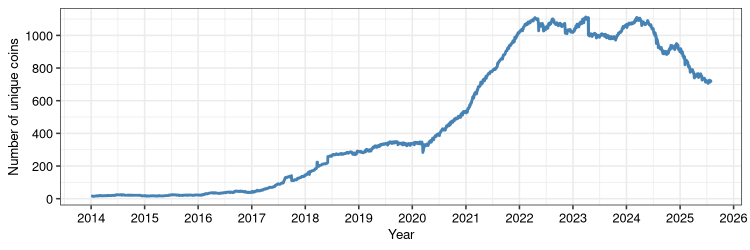
\includegraphics[width=0.8\linewidth,height=\textheight,keepaspectratio]{pictures/timeseries_daily_coins.png}

}

\subcaption{\label{fig-sub1}}

\centering{

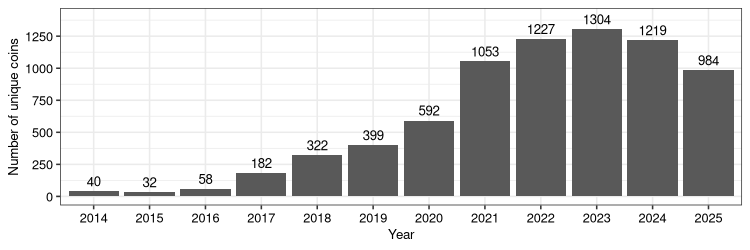
\includegraphics[width=0.8\linewidth,height=\textheight,keepaspectratio]{pictures/coins_per_year.png}

}

\subcaption{\label{fig-sub2}}

}

\caption[Number of cryptocurrencies over
time]{\label{fig-numcoins}\textbf{Number of cryptocurrencies over time.}
Panel A shows the daily time series of the number of unique
cryptocurrencies. Panel B displays the number of unique cryptocurrencies
recorded each year. Both panels correspond to the filtered dataset,
covering the period from January 1, 2014, to July 31, 2025, and
including 1,416 unique cryptocurrencies. Note that coins may enter or
exit the market over time.}

\end{figure}%

\section{Sample overview}\label{sample-overview}

After applying all the filters, the resulting sample consists of 973
unique cryptocurrencies and 1,478,936 observations from June 1, 2018, to
July 31, 2025, where a day starts at 00:00:00 UTC. It is important to
mention that the number of cryptocurrencies fluctuates over the entire
period, which results in an unbalanced panel of data.

\bookmarksetup{startatroot}

\chapter{\texorpdfstring{\texttt{\{r\}\ \#\ \#\textbar{}\ label:\ tbl-summary\ \#\ \#\textbar{}\ echo:\ false\ \#\ \#\textbar{}\ results:\ asis\ \#\ \#\textbar{}\ tbl-cap:\ "Summary\ statistics\ of\ daily\ excess\ returns\ on\ cryptocurrencies\$\^{}\{\textbackslash{}\textbackslash{}dagger\}\$"\ \#\ \ \#\ library(readr)\ \#\ library(xtable)\ \#\ \ \#\ \#\ Read\ your\ pre-formatted\ CSV\ \#\ tbl\_fmt\ \textless{}-\ read\_csv("tables/sample\_overview\_table.csv")\ \#\ \ \#\ \#\ Convert\ to\ data\ frame\ (xtable\ needs\ a\ data.frame,\ not\ tibble)\ \#\ tbl\_fmt\ \textless{}-\ as.data.frame(tbl\_fmt)\ \#\ \ \#\ \#\ Create\ LaTeX\ table\ \#\ latex\_tbl\ \textless{}-\ xtable(\ \#\ \ \ tbl\_fmt,\ \#\ \ \ align\ =\ c("l",\ rep("r",\ ncol(tbl\_fmt))),\ \ \#\ left\ for\ first\ col,\ right\ for\ the\ rest\ \#\ \ \ booktabs\ =\ TRUE\ \#\ )\ \#\ \ \#\ \#\ Print\ LaTeX\ with\ footnote,\ no\ escaping\ \#\ print(\ \#\ \ \ latex\_tbl,\ \#\ \ \ include.rownames\ =\ TRUE,\ \#\ \ \ sanitize.text.function\ =\ identity,\ \ \#\ keep\ \%\ signs\ \#\ \ \ comment\ =\ FALSE\ \#\ )\ \#\ \ \#\ \#\ Footnote\ \#\ \#\ cat("\textbackslash{}\textbackslash{}caption*\{\textbackslash{}\textbackslash{}footnotesize\ \textbackslash{}\textbackslash{}textsuperscript\{\textbackslash{}\textbackslash{}dag\}\ This\ table\ reports\ summary\ statistics\ for\ daily\ excess\ returns.\ The\ columns\ are:\ total\ observations,\ number\ of\ unique\ coins,\ the\ minimum\ cross-sectional\ count\ per\ day,\ the\ mean\ and\ standard\ deviation,\ and\ the\ 10th/25th/50th/75th/90th\ percentiles.\}")\ \#}}{\{r\} \# \#\textbar{} label: tbl-summary \# \#\textbar{} echo: false \# \#\textbar{} results: asis \# \#\textbar{} tbl-cap: "Summary statistics of daily excess returns on cryptocurrencies\$\^{}\{\textbackslash\textbackslash dagger\}\$" \#  \# library(readr) \# library(xtable) \#  \# \# Read your pre-formatted CSV \# tbl\_fmt \textless- read\_csv("tables/sample\_overview\_table.csv") \#  \# \# Convert to data frame (xtable needs a data.frame, not tibble) \# tbl\_fmt \textless- as.data.frame(tbl\_fmt) \#  \# \# Create LaTeX table \# latex\_tbl \textless- xtable( \#   tbl\_fmt, \#   align = c("l", rep("r", ncol(tbl\_fmt))),  \# left for first col, right for the rest \#   booktabs = TRUE \# ) \#  \# \# Print LaTeX with footnote, no escaping \# print( \#   latex\_tbl, \#   include.rownames = TRUE, \#   sanitize.text.function = identity,  \# keep \% signs \#   comment = FALSE \# ) \#  \# \# Footnote \# \# cat("\textbackslash\textbackslash caption*\{\textbackslash\textbackslash footnotesize \textbackslash\textbackslash textsuperscript\{\textbackslash\textbackslash dag\} This table reports summary statistics for daily excess returns. The columns are: total observations, number of unique coins, the minimum cross-sectional count per day, the mean and standard deviation, and the 10th/25th/50th/75th/90th percentiles.\}") \#}}\label{r-label-tbl-summary-echo-false-results-asis-tbl-cap-summary-statistics-of-daily-excess-returns-on-cryptocurrenciesdagger-libraryreadr-libraryxtable-read-your-pre-formatted-csv-tbl_fmt---read_csvtablessample_overview_table.csv-convert-to-data-frame-xtable-needs-a-data.frame-not-tibble-tbl_fmt---as.data.frametbl_fmt-create-latex-table-latex_tbl---xtable-tbl_fmt-align-cl-repr-ncoltbl_fmt-left-for-first-col-right-for-the-rest-booktabs-true-print-latex-with-footnote-no-escaping-print-latex_tbl-include.rownames-true-sanitize.text.function-identity-keep-signs-comment-false-footnote-catcaptionfootnotesize-textsuperscriptdag-this-table-reports-summary-statistics-for-daily-excess-returns.-the-columns-are-total-observations-number-of-unique-coins-the-minimum-cross-sectional-count-per-day-the-mean-and-standard-deviation-and-the-10th25th50th75th90th-percentiles.}

\begin{table}

\caption{\label{tbl-summary}Summary statistics of daily excess returns
on cryptocurrencies}

\centering{

\begin{verbatim}
New names:
Rows: 1 Columns: 11
-- Column specification
-------------------------------------------------------- Delimiter: "," chr
(8): ...1, Mean, Std, P10, P25, P50, P75, P90 dbl (2): Unique coins, Min No.
Obs num (1): No. Obs
i Use `spec()` to retrieve the full column specification for this data. i
Specify the column types or set `show_col_types = FALSE` to quiet this message.
* `` -> `...1`
\end{verbatim}

\centering
\begin{tabular}{lrrrlllllll}
\toprule
...1 & No. Obs & Unique coins & Min No. Obs & Mean & Std & P10 & P25 & P50 & P75 & P90\\
\midrule
Sample & 1478936 & 973 & 121 & -2.70% & 12.49% & -10.18% & -6.65% & -3.70% & 0.02% & 4.69%\\
\bottomrule
\end{tabular}

}

\end{table}%

\section{Characteristic construction and
description}\label{sec-characteristics}

\subsection{Volume shock}\label{volume-shock}

Following Bianchi et al.~(2022), the volume shock is defined as the
log-deviation of trading volume from its rolling average (over 30 or 60
days) for cryptocurrency \(i\) at time \(t\). For \(m \in \{30, 60\}\)
periods, the volume shock is estimated as:

\[
v_{i,t} = \log(\text{Volume}_{i,t}) - \log\left( \frac{1}{m} \sum_{s=1}^{m} \text{Volume}_{i,t-s} \right)
\]

\section{Risk}\label{risk}

\subsection{Realized volatility (rvol)}\label{realized-volatility-rvol}

Using the volatility estimator of Yang and Zhang (2000), I compute the
daily realized volatility based on OHCL prices over a rolling 30-day
window. For \(n > 1\) number of periods, the volatility estimate at time
\(t\) is:

\[
\sigma_t = \sqrt{\sigma^2_O + k\sigma^2_C + (1 - k)\sigma^2_{RS}}
\] where \(\sigma^2_{RS}\) is the variance estimator of Rogers et
al.~(1994), and \(\sigma^2_O\), \(\sigma^2_C\), \(k\) are defined as
follows:

\[
\sigma^2_O = \frac{1}{n-1}\sum\limits_{i=1}^n(o_i - \bar o)^2,
\]

\[
\sigma^2_C = \frac{1}{n-1}\sum\limits_{i=1}^n(c_i - \bar c)^2,
\]

\[
k = \frac{\alpha -1}{\alpha + \frac{n+1}{n-1}}
\]

with \(o = ln\,O_t - ln\,C_{t-1}\), and \(c = ln\,C_t - ln\,O_t\). Here,
\(C_{t-1}\) denotes the last days' closing price and \(O_t\) the current
day's opening price. I set the constant \(\alpha = 1.34\) as suggested
by Yang and Zhang (2000) to be the best value in practice.

Moskowitz et al. (2012)

This is more related to factor construction.

Organize week in the following way: the first seven days of the year
forms the first week, and the first 51 weeks of the year consists of 7
days each. The 52th week of the year consists of the last eight days
and, in case of a leap year (as 2016, 2020, and 2024), of nine days.

Similar to \textbf{Liu et al}, I construct a daily cryptocurrency market
return as the value-weighted average return of all the cryptocurrencies
in the sample. For cryptocurrencies \(i = 1, ..., N\), the daily market
return at time \(t\) is computed as:

\[
r_t^M = \frac{\sum_{i=1}^N r_{it} \cdot marketcap_{it}}
             {\sum_{i=1}^N marketcap_{it} }
\]

The cryptocurrency market excess return (\texttt{CMKT}) is constructed
as the difference between the cryptocurrency market return and the
risk-free rate. To proxy the risk-free rate, I used the (daily) 1-month
Treasury bill rate from the FRED.

Write this in the following section of ``Empirical application'' or This
is for the model: 7. (Still undecisive) Minimum cross-section. Following
the criterion by Kelly, I Convert variables in the -0.5 - 0.5 range

The sample period ranges from January 1st, 2014, to May 31st, 2025.

\bookmarksetup{startatroot}

\chapter*{References}\label{references}
\addcontentsline{toc}{chapter}{References}

\markboth{References}{References}

\phantomsection\label{refs}
\begin{CSLReferences}{1}{0}
\bibitem[\citeproctext]{ref-asadovGreaterStability2023}
Asadov, A., Yildirim, R., \& Masih, M. (2023). Toward greater stability
in stablecoins: Empirical evidence from an analysis of precious metals.
\emph{Borsa Istanbul Review}, \emph{23}(5), 1152--1172.
\url{https://doi.org/10.1016/j.bir.2023.07.004}

\bibitem[\citeproctext]{ref-baurCryptoSafe2021}
Baur, D. G., \& Hoang, L. T. (2021). A crypto safe haven against
Bitcoin. \emph{Finance Research Letters}, \emph{38}, 101431.
\url{https://doi.org/10.1016/j.frl.2020.101431}

\bibitem[\citeproctext]{ref-bianchiMispricingRiskCompensation2021}
Bianchi, D., \& Babiak, M. (2021). \emph{Mispricing and Risk
Compensation in Cryptocurrency Returns} (SSRN Scholarly Paper 3935934).
Social Science Research Network.
\url{https://doi.org/10.2139/ssrn.3935934}

\bibitem[\citeproctext]{ref-chamberlainArbitrageFactor1983}
Chamberlain, G., \& Rothschild, M. (1983). Arbitrage, Factor Structure,
and Mean-Variance Analysis on Large Asset Markets. \emph{Econometrica},
\emph{51}(5), 1281--1304. \url{https://doi.org/10.2307/1912275}

\bibitem[\citeproctext]{ref-chenOpenSource2021}
Chen, A. Y., \& Zimmermann, T. (2021). \emph{Open Source Cross-Sectional
Asset Pricing} (SSRN Scholarly Paper 3604626). Social Science Research
Network. \url{https://doi.org/10.2139/ssrn.3604626}

\bibitem[\citeproctext]{ref-chenSemiparametricConditional2022}
Chen, Q., Roussanov, N. L., \& Wang, X. (2022). \emph{Semiparametric
Conditional Factor Models in Asset Pricing} (SSRN Scholarly Paper
3984633). Social Science Research Network.
\url{https://doi.org/10.2139/ssrn.3984633}

\bibitem[\citeproctext]{ref-chenCommonRisk2024}
Chen, Z., Roussanov, N. L., Wang, X., \& Zou, D. (2024). \emph{Common
Risk Factors in the Returns on Stocks, Bonds (and Options), Redux} (SSRN
Scholarly Paper 4703281). Social Science Research Network.
\url{https://doi.org/10.2139/ssrn.4703281}

\bibitem[\citeproctext]{ref-coinbaseWhatWrapped}
Coinbase. (n.d.). \emph{What is wrapped crypto?} Retrieved August 6,
2025, from
\url{https://www.coinbase.com/learn/your-crypto/what-is-wrapped-crypto}

\bibitem[\citeproctext]{ref-connorPerformanceMeasurement1986}
Connor, G., \& Korajczyk, R. A. (1986). Performance measurement with the
arbitrage pricing theory: A new framework for analysis. \emph{Journal of
Financial Economics}, \emph{15}(3), 373--394.
\url{https://doi.org/10.1016/0304-405X(86)90027-9}

\bibitem[\citeproctext]{ref-famaCommonRisk1993}
Fama, E. F., \& French, K. R. (1993). Common risk factors in the returns
on stocks and bonds. \emph{Journal of Financial Economics},
\emph{33}(1), 3--56. \url{https://doi.org/10.1016/0304-405X(93)90023-5}

\bibitem[\citeproctext]{ref-famaFivefactorAsset2015}
Fama, E. F., \& French, K. R. (2015). A five-factor asset pricing model.
\emph{Journal of Financial Economics}, \emph{116}(1), 1--22.
\url{https://doi.org/10.1016/j.jfineco.2014.10.010}

\bibitem[\citeproctext]{ref-financialstabilityboardAddressingRegulatory2020}
Financial Stability Board. (2020). \emph{Addressing the regulatory,
supervisory and oversight challenges raised by {``global stablecoin''}
arrangements: Consultative document}.
\url{https://www.fsb.org/2020/04/addressing-the-regulatory-supervisory-and-oversight-challenges-raised-by-global-stablecoin-arrangements-consultative-document/}

\bibitem[\citeproctext]{ref-hoangHowStable2024}
Hoang, L. T., \& Baur, D. G. (2024). How stable are stablecoins?
\emph{The European Journal of Finance}, \emph{30}(16), 1984--2000.
\url{https://doi.org/10.1080/1351847X.2021.1949369}

\bibitem[\citeproctext]{ref-kellyCharacteristicsAre2019}
Kelly, B. T., Pruitt, S., \& Su, Y. (2019). Characteristics are
covariances: A unified model of risk and return. \emph{Journal of
Financial Economics}, \emph{134}(3), 501--524.
\url{https://doi.org/10.1016/j.jfineco.2019.05.001}

\bibitem[\citeproctext]{ref-liuCommonRisk2022}
Liu, Y., Tsyvinski, A., \& Wu, X. (2022). Common Risk Factors in
Cryptocurrency. \emph{The Journal of Finance}, \emph{77}(2), 1133--1177.
\url{https://doi.org/10.1111/jofi.13119}

\bibitem[\citeproctext]{ref-mercikCrosssectionalInteractionsCryptocurrency2025}
Mercik, A., Będowska-Sójka, B., Karim, S., \& Zaremba, A. (2025).
Cross-sectional interactions in cryptocurrency returns.
\emph{International Review of Financial Analysis}, \emph{97}, 103809.
\url{https://doi.org/10.1016/j.irfa.2024.103809}

\bibitem[\citeproctext]{ref-moskowitzTimeSeriesMomentum2012}
Moskowitz, T. J., Ooi, Y. H., \& Pedersen, L. H. (2012). Time series
momentum. \emph{Journal of Financial Economics}, \emph{104}(2),
228--250. \url{https://doi.org/10.1016/j.jfineco.2011.11.003}

\bibitem[\citeproctext]{ref-wangAreStablecoins2020}
Wang, G.-J., Ma, X., \& Wu, H. (2020). Are stablecoins truly
diversifiers, hedges, or safe havens against traditional
cryptocurrencies as their name suggests? \emph{Research in International
Business and Finance}, \emph{54}, 101225.
\url{https://doi.org/10.1016/j.ribaf.2020.101225}

\end{CSLReferences}




\end{document}
